\documentclass[]{article}
\usepackage{color}
\usepackage{graphicx}
%\usepackage{bib}
%opening
\title{Few-shot generation of images of products with defects by fine-tuning large diffusion models}
\author{Avadhut Sardeshmukh}

\begin{document}

\maketitle

\section{Problem Statement}
Asset maintenance and inspection are critical components of operating power lines and substations. Performing these tasks at scale—across thousands of kilometers of infrastructure—poses significant challenges. Early detection of visible degradation, faults, or other anomalies can lead to substantial cost savings and improved system reliability. However, a key obstacle is the limited availability of anomalous image data for each defect type. 

To address this, one promising approach is to augment training data using synthetic images. Toward this end, the present task is to create a conditional image generation model for this purpose by fine-tuning a pre-trained diffusion model on limited labeled data of the target product and defects. 

\section{Possible Solutions}
Conditional image generation is a fundamental problem in computer vision, and has received a lot of attention in recent research. With the rise of models such as generative adversarial networks (GANs) and variational autoencoders (VAEs), deep generative models started showing promise for synthetic image generation. While VAEs model and optimize the data likelihood explicitly, GANs do this implicitly through an adversarial network, leading to sharper images with better perceptual quality. GANs quickly became popular and were adapted for diverse applications (such as generating synthetic speech data and e-commerce visuals). However, GANs are known to be notoriously difficult to train because of the underlying mini-max game. A flurry of research addressed the problems of GAN training stability and other issues such as mode-collapse (e.g. WGAN, WGAN-GP, SpectralNormGAN and so on). Meanwhile, with the advent of better compute and learning architectures, the liklihood (and score)-based modeled regained the attention, resulting in the recent advances in diffusion models. Latest diffusion models such as DDPM, GLIDE, Imagen, ControlNet, and Stable Diffusion 3 are very powerful image generators. While the original DDPM model was unconditional, the follow-up research effectively addressed the problem of conditioning through various ways : 
\begin{itemize}
	\item Adding the conditioning information as extra channels in the ResNet blocks
	\item Combining conditioning information with timesteps in diffusion
	\item Using the gradients from a separately trained classifier
	\item Guidance (e.g. Contrastive Language-Image Pretraining Guidance for alignment with text)
	\item Classifier free guidance 
\end{itemize}
These models have internalized various semantics of different image types through their extensive training on millions (or even billions in some cases, such as SD3) of images with and without labels. They make a very good choice for making a model for few-shot image generation on a new class of images. 

\subsection{Fine-tuning methods}
Some possible ways to fine tune these pre-trained models for our task are :
\begin{enumerate}
	\item Full fine-tuning\\
	The huge parameter space of these models poses a significant challenge in full fine-tuning since the optimizer needs to maintain the state of all the parameters, requiring large GPU memory.
	\item Parameter efficient fine-tuning\\
	Much of recent literature on synthetic image generation for various applications has focused on parameter efficient fine-tuning methods. The notable ones among these include tuning just the biases (BitFit~\cite{bitfit}), tuning based on prompts (VPT~\cite{vpt}), low-rank adaptation methods from the language modeling literature (LoRA~\cite{lora}, DriveDitFit~\cite{driveditfit}), and tuning biases and newly added scales (DiffFit~\cite{difffit}).
	\item Augmenting model's conditioning space\\
	This class of methods is particularly suitable for fine-tuning text-conditional models such as stable diffusion. They are based on the idea of creating new "words" in the embedding space which correspond to new concepts. Most notable approaches include Dreambooth~\cite{dreambooth} and Textual Inversion~\cite{textualinversion}. 
	\item Distillation\\
	These methods train smaller models by leveraging the training signal from the large models, effectively ``distilling'' the knowledge contained in the larger models. 
\end{enumerate}
\section{Modeling and Implementation}
\subsection{Modeling Considerations}
\subsubsection{Diffusion Model}
The task includes class-conditional generation of defective product images. Unconditional models such as DDPM and DDIM are not directly useful here. Further, the latest models such as Imagen, Glide and SD3 are text conditional, so adapting them for this task is not as straightforward. Instead, a recent model from facebook research, called diffusion transformer (DiT), based on the vision transformer (ViT) architecture and trained on the Imagenet dataset for class-conditional generation, is better suited for our task. I chose to fine-tune one of the two largest DiT models, \textbf{DiT-XL-2-256}, which are available in the huggingface diffusers pipeline.
\subsubsection{Data - The Product Type}
The suggested dataset, DefectSpectrum, contains images of various product types such as \texttt{pill}, \texttt{zipper}, \texttt{hazelnut}, \texttt{metal nut} and \texttt{screw}. For each product, there can be a number of defect types (e.g., for \texttt{hazelnut}, the defects are \texttt{hole},\texttt{crack},\texttt{cut}, $\ldots$). There is a set of images (typically ~20) of each product-defect combination. The present task is to choose any one product type and then treat the defect types as classes for class-conditional generation. I chose to experiment with \texttt{hazelnut} and \texttt{screw}. One of the main reasons behind this particular choise is that there are similar class labels in Imagenet (\texttt{buckeye} and \texttt{screw}, respectively), and so the learned class embeddings for these classes can perhaps be fine-tuned easily. 
\section{Experiments}
\subsection{Fine Tuning}
\subsubsection{Choosing Parameters}
I first implemented a finetuning function using the diffusers implementation of DiTs and the pre-trained weights of DiT-XL-2-256. However, this required a lot of GPU memory, often running into OOM errors. Also, given the small amount of tuning data, full fine-tuning wouldn't be feasible. 

I went through some of the parameter efficient fine-tuning methods and found that BitFit and DiffFit were the most suited for this task. BitFit was originally proposed for fine-tuning language models, and the idea of tuning just the biases was extended in DiffFit, where, in addition to the biases, they also tune the kayer norm weights, class embeddings, and learn new scale parameters for each DiT block.  

Adapting from DiffFit, \textbf{\textcolor{red}{I selected all the biases and layernorm weights for tuning, without adding new scale parameters. In the huggingface implementation, the layernorm includes class label embeddings too.}}

Tuning the class embeddings is perhaps the most important thing since the association of the class labels with Imagenet classes must now be changed to reflect the new classes. \textcolor{red}{\textbf{I chose those product types for which a similar class label was available in Imagenet} - for example, screw. And I started the class IDs at the index of this label. My hypothesis is that \textbf{in this case, the class embeddings can to be tuned relatively easily.}}
\subsection{Choosing Hyperparameters}
\begin{enumerate}
	\item \textbf{Batch Size} - I used very small batch sizes (tried 1, 2, 4, and 8) to avoid OOM errors and also because the dataset is quite small. With larger batch sizes, I slightly increased the learning rate. However, smaller batch sizes worked better. In particular, batch size 8 resulted in unstable training. 
	\item \textbf{Learning Rate} - I used small learning rate values. I tried $1e-6, 1e-5, 2e-5$ and $3e-5$. Of these, training with $1e-5$ was more stable. With $3e-5$ I got one of the best samples, but the training collapsed after 50 epochs. 
	\item \textbf{Gradient Accumulation} - Since the batch sizes were very small, I used  gradient\_accumulation\_=2. That is, the gradients are accumulated for two steps before applying the weight updates. This gives the benefits of large batches while using small batch sizes. 
	\item \textbf{Noise Scheduler Steps} - The number of of noise scheduler steps in inference (the training steps are fixed. I observed that more steps ($>100$) worked better, but only upto an extent (tried 200, 500); $1000$ was worse. 
	\item \textbf{Mixed Precision Training} for memory efficiency. Torch automatically applies the optimal precision (autocast), such as fp16 or fp32 to each parameter, allowing mixed precision training. 	
\end{enumerate}
\subsection{Data Preprocessing and Augmentation}
\begin{enumerate}
	\item \textbf{Image Size}\\
	Experimented with 256, 128 and 64. While training with small image size is lighter on the memory, making it possible to use large batches (upto 8), I observed it worked better with 128. This could be because the model was originally trained on 256x256 images. 
	\item \textbf{Normalization}\\
	Following the normalization scheme in the original paper, I scaled the pixel values in the range $[-1,1]$.
	\item \textbf{Preprocessing}\\
	For \texttt{hazelnut}, since there was a lot of black background in these images, I cropped the center 800x800 (original images were 1024x1024), and then resized to desired resolution. This was not required for \texttt{screw}.
	\item \textbf{Augmentation}\\
	I applied the transforms RandomHorizontalFlip, RandomVerticalFlip and RandomRotation (with degree in $[45,65,120]$ which is quite different from Flip). These are applied randomly to each image each time, resulting in variation in the data in each epoch, allowing to train for more epochs
	\item \textbf{Epochs}\\
	First I trained a model with any new config for 10 epochs, to see if it's working. If yes, then I trained it for 100 epochs. Also tried to implement early stopping (based on just the training loss), but this wasn't working as epected. 
\end{enumerate}
\subsection{Results}
The best generated samples for hazelnut and screw are shown below. Columns correspond to class labels and rows are different samples.\\ 
\begin{center}
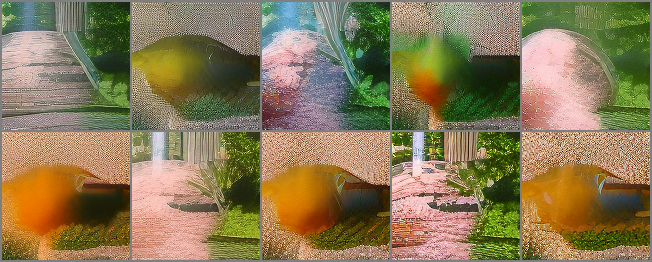
\includegraphics[scale=0.2]{hazelnut}\\
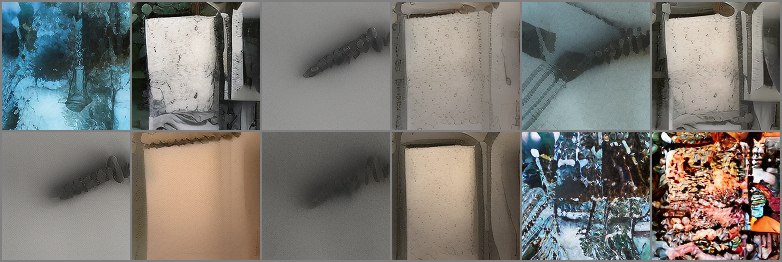
\includegraphics[scale=0.2]{screw}\\
\end{center}
\section{Evaluation Metrics}
\begin{enumerate}
	\item  Class-wise FID and Inception score
	\item Improvement in accuracy of the downstream task model with generated data (various metrics of the downstream model such as accuracy, f1, precision, recall, mAP\@x\% can be used).  
\end{enumerate}
\section{Further Scope}
\subsection{Model Improvements}
Given more time, following two things can possibly lead to substantially better generations:
\begin{enumerate}
	\item The huggingface implementation of DiT hides the hyperparameters such as classifier free guidance in the long class hierarchy. While classifier free guidance scale has been implemented, their DiT class does not implement a "forward\_with\_cfg" method. Instead, one can work with the original codebase to tune and gain more control over all the hyperparameters
	\item A recent paper DriveDitFit~\cite{driveditfit} proposed a LoRA fine-tuning method for DiT. They propose to replace the class embeddings with closest Imagenet class-embeddings according to a CLIP similarity between corresponding images. This can be used to get good initialization for the class embeddings. 
	\item Other LoRA approaches of fine-tuning and knowledge distillation.
\end{enumerate}
\subsection{Leveraging Extra Information}
The DefectSpectrum dataset also includes segmentation masks that demarcate the defects on the product image (e.g. hole in hazelnut). These segmentation masks are images of the same size as the original images. The masks can be used as extra conditional information in addition to the class label and timestep. The recent ControlNet architecture~\cite{controlnet} supports conditioning on an image. This could be a very useful guidance for generating small defects, which otherwise could be difficult to generate. 
\bibliographystyle{unsrt}
\bibliography{refs}
\end{document}
